\begin{figure}[!t]
\centering
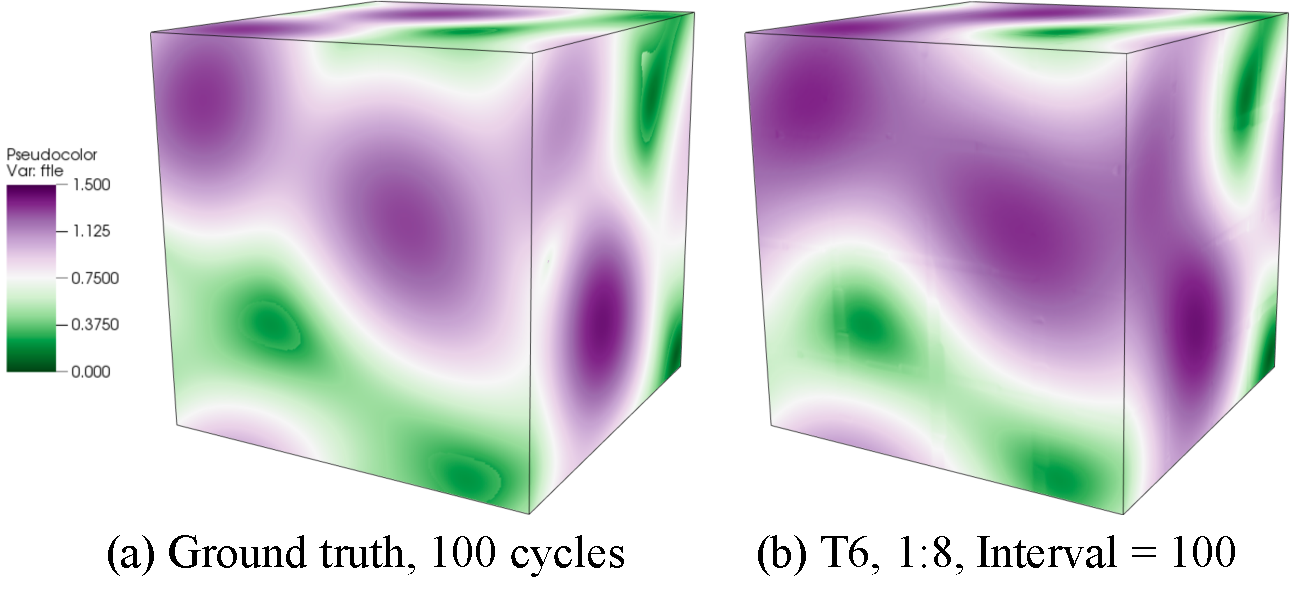
\includegraphics[width=\linewidth,keepaspectratio]{Images/abc_ftle_new3.pdf}
\caption{\fix{3D colormapped surfaces of the FTLE field for the ABC data set. While the FTLE field derived using the reduced Lagrangian$_{Local}$ flow map~(right) maintains the overall structure, some information is lost along node boundaries.}}
%\caption{A comparison of colormapped surface of a subvolume of FTLE scalar fields generated post hoc using the flow maps of Lagrangian$_{Dist}$~(left) and Lagrangian$_{Local}$~(right). Ridges in the FTLE field (identified by high scalar values), are used to visualize regions of interest. Cyan boxes highlight visible instances of difference in the output.}}
\label{abc_ftle}
\vspace{-4mm}
\end{figure}
